\section{Analyse des Schaltplans vom Empfänger} %Erik
\begin{figure}[H]
    \centering
    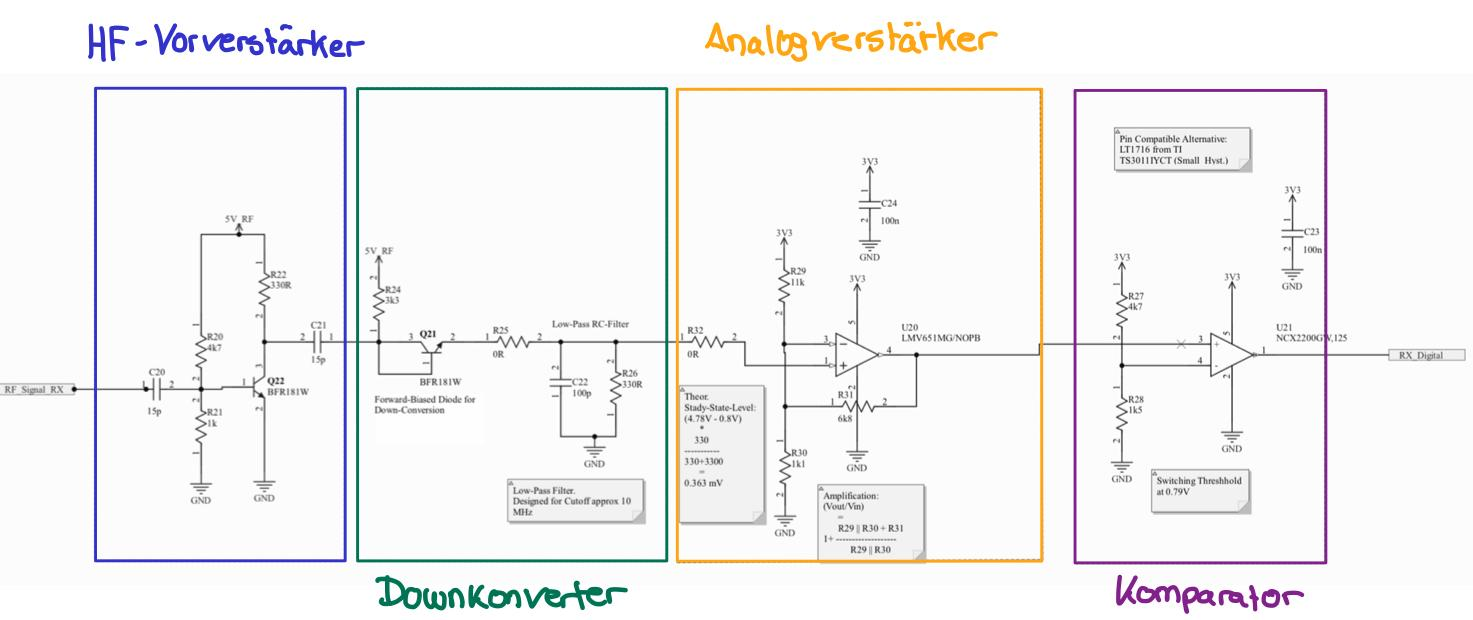
\includegraphics[width=1\textwidth]{Pictures/Schaltbild.jpg}
    \caption{Schaltplan des Empfängers}
    \label{fig:opamp_schaltung}
\end{figure}
Der Empfänger setzt sich aus mehreren Funktionsblöcken zusammen, die das hochfrequente analoge Signal empfangen, vorverstärken,
demodulieren, die niederfrequenten Anteile verstärken und anschließend in ein digitales Signal umwandeln. Da in Versuch 4 bereits auf den
Schaltplan des Empfängers eingegangen wurde, werden hier nur grob die Funktionsblöcke erläutert und hiermit auf das zuvor abgegebene Protokoll verwiesen.
Es folgt jedoch im Rahmen des Versuches noch eine genauere Betrachtung von einzelnen Komponenten. 
\clearpage
Der erste Funktionsblock ist der Hochfrequenzvorverstärker. Er besteht aus einer einfachen Transistorschaltung (u. a), um das durch die Übertragung
geschwächte Signal auf ein nutzbares Niveau zu bringen. \\\\
Der zweite Funktionsblock ist der Downkonverter. Er besteht aus einem HF-Gleichrichter und einem RC-Tiefpass. Der Zweck ist
die Umwandlung des hochfrequenten Signals in ein niederfrequentes Signal und der folgende Tiefpass unterdrückt die hochfrequente Trägerwelle.
\\\\
Es folgt der Analogverstärker bestehend aus einem Operationsverstärker (u. a.). Er dient dazu, das niederfrequente Signal
auf ein geeignetes Niveau zur digitalen Weiterverarbeitung zu bringen.\\ \\
Der letzte Funktionsblock ist der Komparator. 
Der Komparator wandelt das analoge Signal in ein digitales Signal um, welches von einem Computer weiterverarbeitet werden kann. 



\section{Vorverstärkung des Signals} %Lukas
Die Friis-Formel ist eine wichtige Formel in der Nachrichtentechnik, um die Rauschzahl SNR einer Kette von Verstärkern
bzw. Dämpfungsgliedern zu berechnen.

\begin{figure}[H]
    \centering
    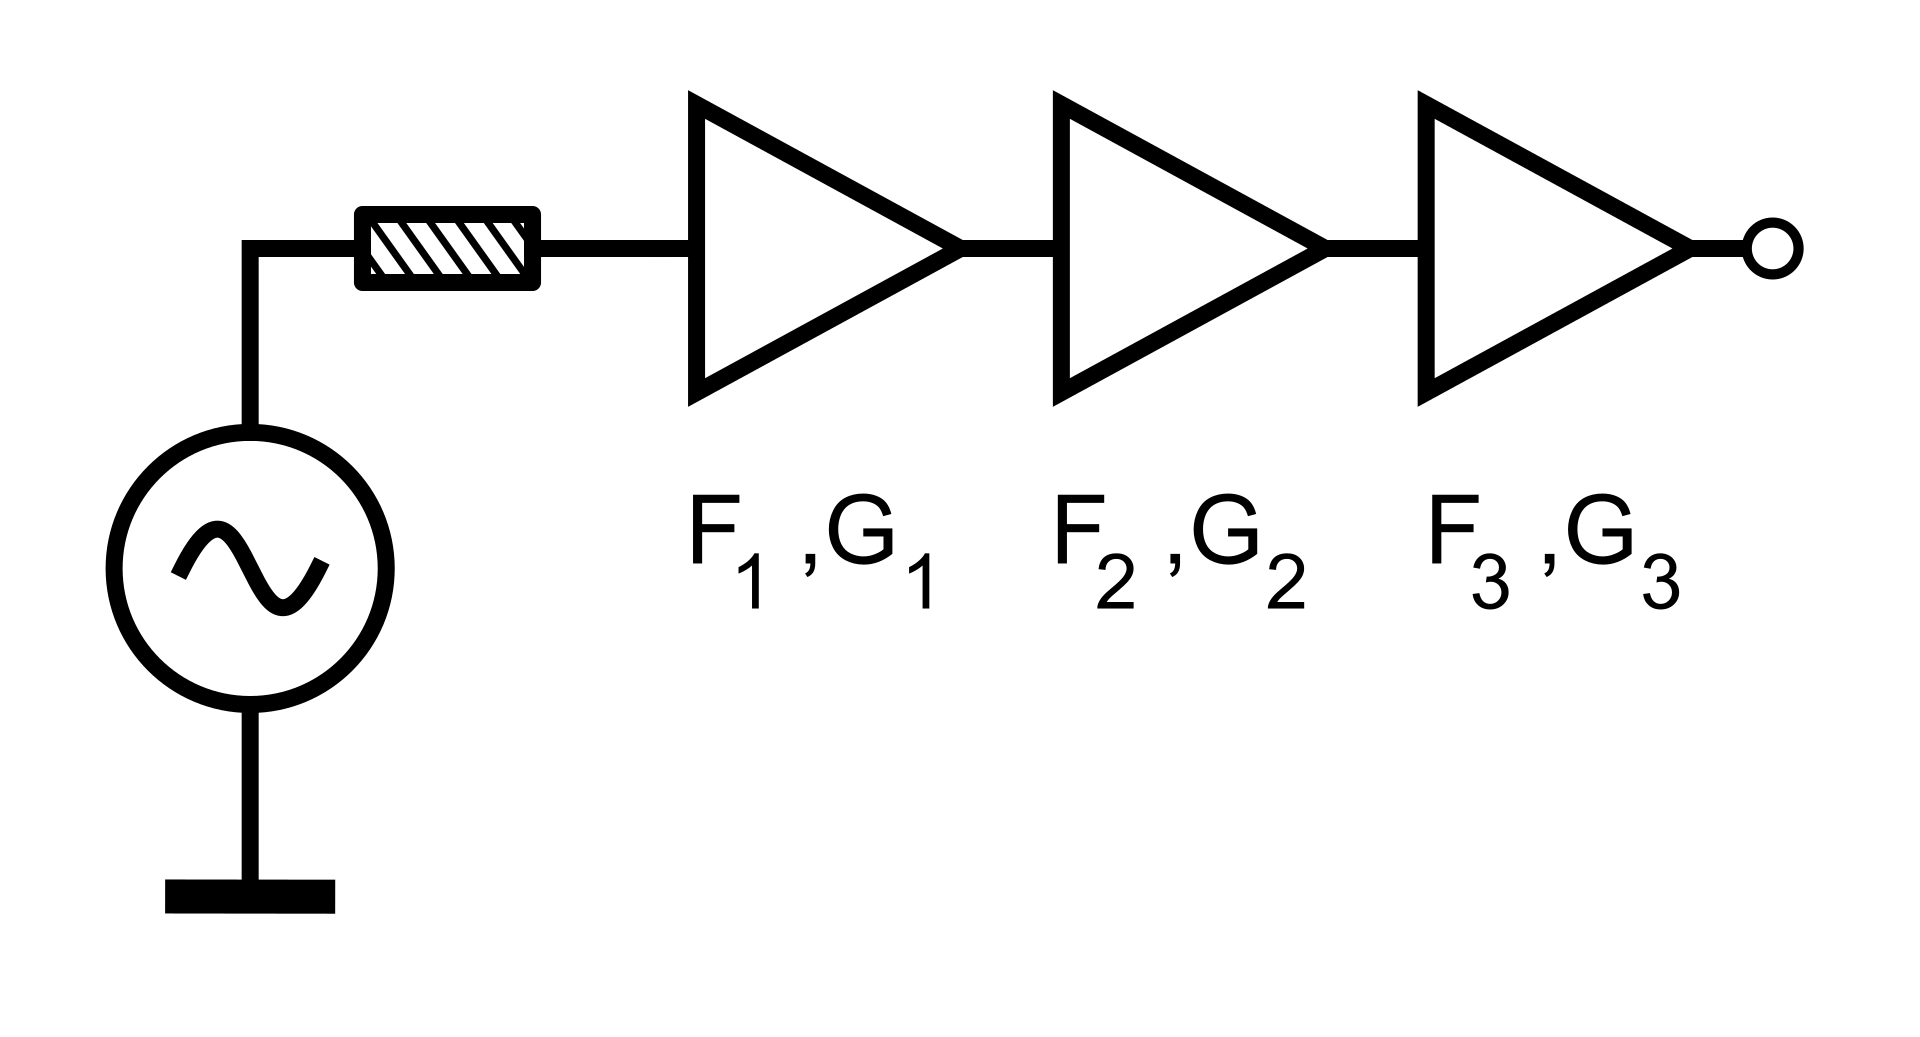
\includegraphics[width=0.4\textwidth]{Pictures/Frijs-Kette.svg.png}
    \caption{Verstärkerkette}
    \footnotesize{Quelle: \url{https://de.wikipedia.org/wiki/Friis-Formel#/media/Datei:Frijs-Kette.svg}}
    %\label{fig:link_budget}
\end{figure}
Für eine Verstärkerkette mit $n$ Verstärkern ergibt sich die Rauschzahl folgendermaßen:
\begin{equation}
    F_{\text{gesamt}} = 1 + (F_1 - 1) + \frac{F_2 - 1}{G_1} + \frac{F_3 - 1}{G_1 G_2} + \frac{F_4 - 1}{G_1 G_2 G_3} + \dots + \frac{F_n - 1}{G_1 G_2 G_3 \dots G_{n-1}}
\end{equation}
\begin{itemize}
    \item $F_{\text{gesamt}}$: Die Gesamte Rauschzahl der Verstärkerkette
    \item $F_i$: Die Rauschzahl des $i$-ten Verstärkers
    \item $G_i$: Die Verstärkung des $i$-ten Verstärkers
\end{itemize}
Es wird schnell ersichtlich, dass Verstärker am Anfang der Kette den meisten Einfluss auf die Gesamtrauschzahl haben.
Deswegen sollten die Verstärker mit der höchsten Verstärkung immer am Anfang der Kette stehen. Andersherum sollten Bauteile mit Dämpfung am Ende der Kette stehen.
\\
Deshalb sollte ein Signal immer zuerst vorverstärkt werden, bevor die Frequenzkonversion durchgeführt wird.
Würde das Signal zuerst gemischt und dann nachverstärkt werden, hätten wir im Vergleich ein deutlich höheres Rauschen,
da der Verstärker im Vergleich zum Mischer eine höhere Verstärkung hat. Je nach Mischer kann dieser sogar auch dämpfend wirken.
\section{Frequenz-Downkonversion} %Farhad
Im Folgenden wird die Frequenz-Downkonversion des analogen Signals erklärt, das bereits vor dem Eingang in den Downkonverter verstärkt wurde.
\subsection{Ablauf der Frequenz-Downkonversion in der Schaltung}
In Abbildung \ref{fig:downconverter} ist die Schaltung des Downkonverters zu sehen.
\begin{figure}[H]
    \centering
    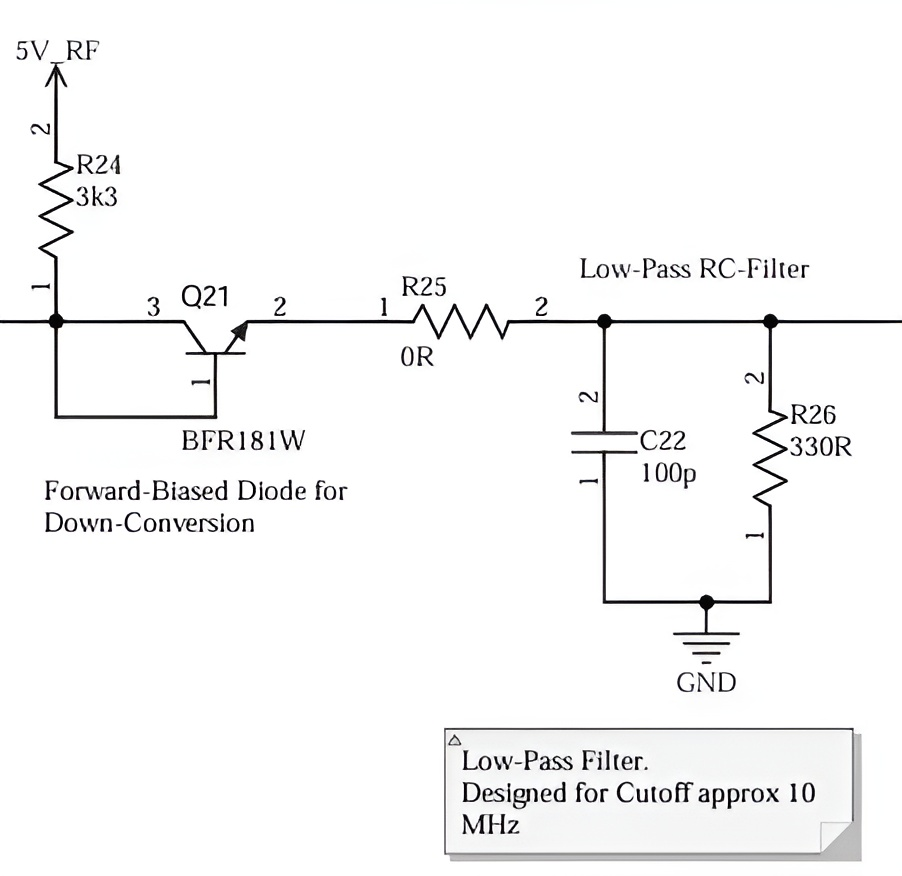
\includegraphics[width=0.6\textwidth]{Pictures/Downconverter.png}
    \caption{Schaltung des Downkonverters}
    \label{fig:downconverter}
\end{figure}
Ein Downkonverter stellt einen einfachen Abwärtsmischer dar, der dazu dient, ein hochfrequentes Eingangssignal in ein niederfrequentes Ausgangssignal umzuwandeln. 

Zuerst gelangt das hochfrequente Signal in den Transistor Q21 (BFR181W), der in diesem Fall nicht als Verstärker, sondern als Diode betrieben wird, da Basis und Kollektor miteinander verbunden sind. Somit wird effektiv nur die Basis-Emitter-Strecke des Transistors benutzt. Der Transistor ist ein \textbf{nichtlineares} Bauelement.
Ein nichtlineares Bauelement wird zum Mischvorgang in diesem Zusammenhang benötigt, da es die Amplitudendemodulation des Signals ermöglicht. 

An den Eingang des Mischers, also des Transistors Q21, werden normalerweise zwei Signale angelegt: das eigentliche \ac{RF}-Signal, welches in diesem Fall bei 1,25 GHz liegt, und ein \ac{LO}-Signal.

Wenn die beiden Signale die vorgespannte Diode passieren, erzeugen diese aufgrund der nichtlinearen Eigenschaften des Transistors eine Mischung der beiden Signale. Die neuen Frequenzen sind hierbei die Summe $f_{RF} + f_{LO}$ und die Differenz $f_{RF} - f_{LO}$ der Eingangsfrequenzen. 

Nach der erfolgreichen Abwärtsmischung des Signals kommt es zu einer Signalfilterung. Dazu wird direkt nach dem Transistor Q21 ein RC-Tiefpassfilter geschaltet, der die Frequenz $f_{RF} + f_{LO}$ herausfiltert und nur das niederfrequente Differenzsignal $f_{RF} - f_{LO}$ passieren lässt. Der Filter besteht aus den Bauelementen R26 ($330~\Omega$) und C22 ($100~\mathrm{pF}$). Der Kondensator ist dabei so dimensioniert, dass der Filter insgesamt eine Grenzfrequenz von $f_{c} = 10~\mathrm{MHz}$ aufweist. Dies widerspricht zwar dem rechnerischen Wert, der sich aufgrund der Werte von R26 und C22 ergibt, also:
\begin{equation}
    f_{c, \text{rechnerisch}} = \frac{1}{2\pi R C}
\end{equation}
Dies lässt sich jedoch durch Vereinfachungen im Schaltplan oder die Tatsache, dass hier ein idealer Tiefpassfilter angenommen wird, erklären. Außerdem ist es bei hohen Frequenzen zu beachten, dass die Leiterbahnen in der Schaltung parasitäre Effekte aufweisen (in Form von Induktivitäten und Kapazitäten), die ebenfalls die Grenzfrequenz beeinflussen können. Diese wurden in der oben ausgeführten Berechnung nicht berücksichtigt.

Jedoch liegt in diesem Fall ein passiver Abwärtsmischer vor, da hier kein \ac{LO} zur Anwendung kommt. Trotzdem funktioniert die Abwärtsmischung des Signals, da der Transistor Q21, wie bereits erklärt, ein nichtlineares Bauelement ist.

\subsection{Funktion des Widerstands R\textsubscript{24}}
Die Widerstände R24 und R26 bilden einen Spannungsteiler, der den Arbeitspunkt des Transistors Q21 festlegt. Hierbei sollte der Arbeitspunkt durch die Widerstände R24 und R26 so gewählt werden, dass der Transistor eine möglichst starke Krümmung auf der Kennlinie im Arbeitspunkt aufweist und damit stark nichtlinear ist. Dadurch wird eine optimale Signalverarbeitung ermöglicht, da der Transistor in der Lage ist, das Signal richtig zu demodulieren und weiterzuleiten. Ohne R24 könnte der Transistor übersteuert werden, was zu Verzerrungen im Signal oder zur Zerstörung des Transistors führen würde.
Durch die Vorspannung des Transistors Q21 über den Widerstand R24 wird der Transistor Q21 knapp unterhalb seines leitenden Bereichs betrieben, sodass er für kleinere Signale empfindlich ist. Das hat eine Verbesserung der Mischungseigenschaften des Transistors zur Folge.

\section{Operationsverstärkerschaltung} %Lukas 5a und c
Der Operationsverstärker, der im PCB des Praktikums verbaut ist, ist hier zu sehen:
\begin{figure}[H]
    \centering
    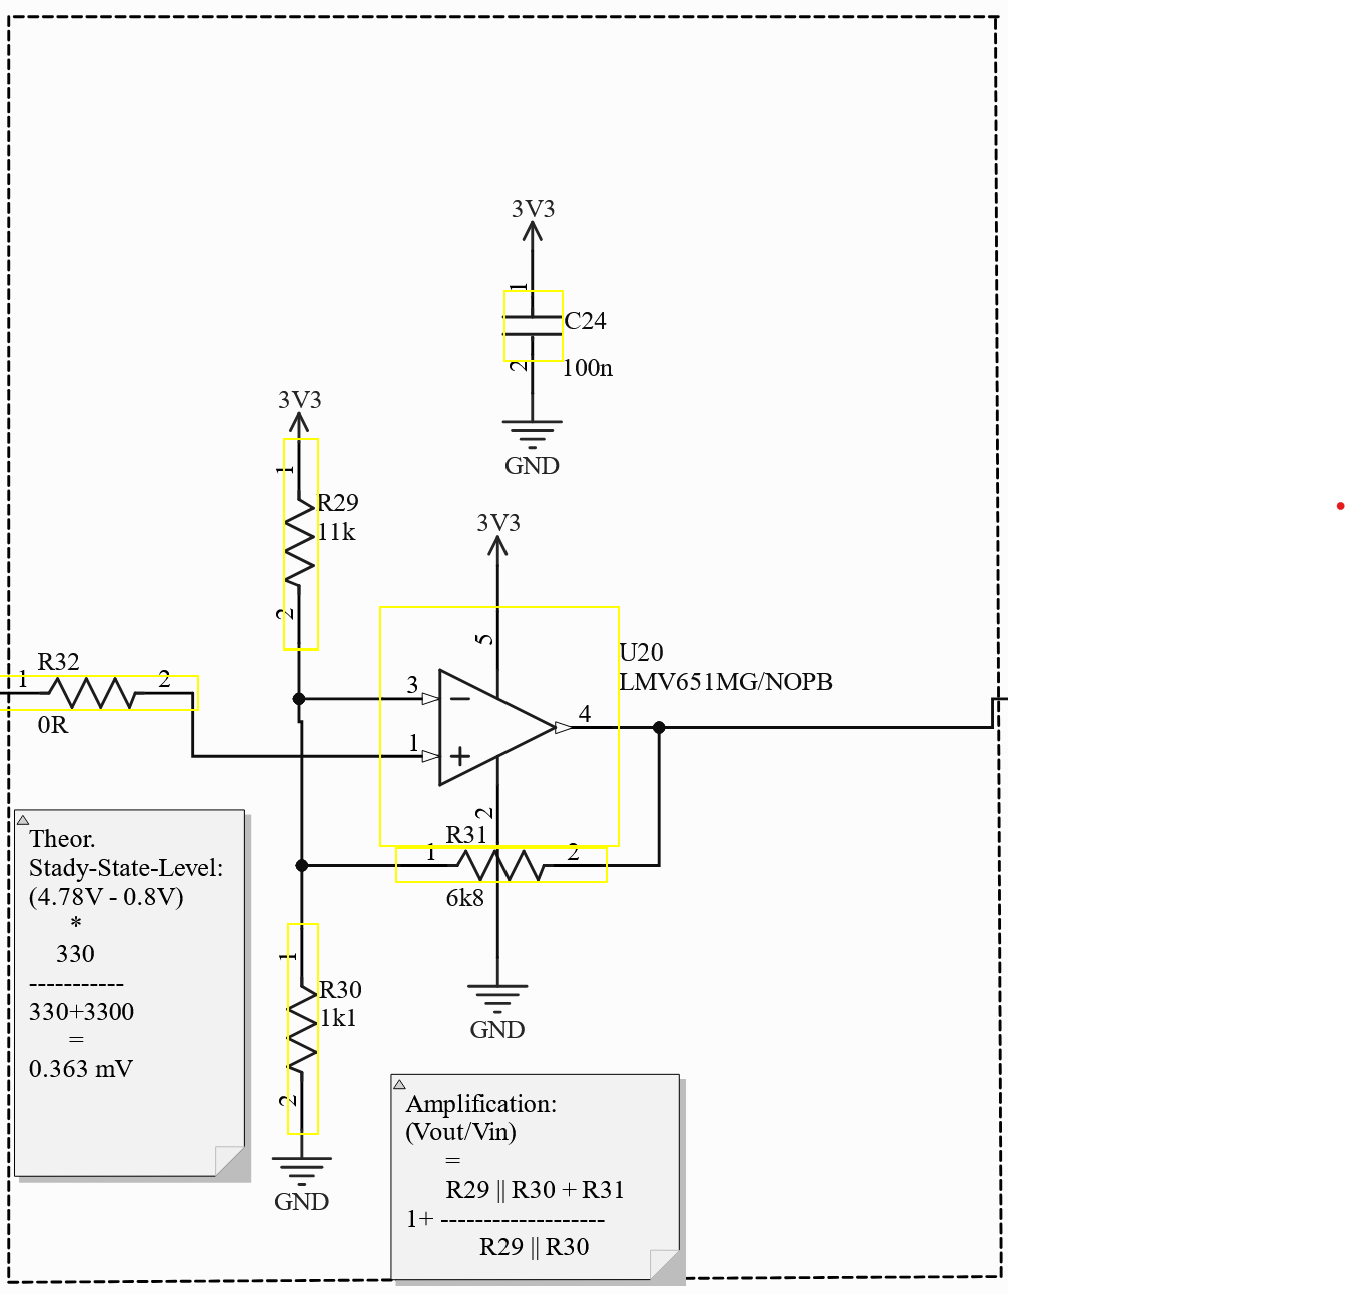
\includegraphics[width=0.8\textwidth]{Pictures/OP_Verstaerker.png}
    \caption{Operationsverstärkerschaltung}
    \label{fig:opamp_schaltung}
\end{figure}
Es handelt sich um einen nichtinvertierenden Operationsverstärker.
Für die Übertragung eines generellen nichtinvertierenden Operationsverstärkers gilt:
\begin{equation}
    \frac{U_{out}}{U_{in}} = 1 + \frac{R_f}{R_{in}}
\end{equation}
Für die gegebene Schaltung in Abbildung 2.4 gilt:
\begin{itemize}
    \item $R_f$: Widerstand zwischen Ausgang und invertierendem Eingang ($R_{31}$)
    \item $R_{in}$: Paralleler Ersatzwiderstand $R_{29}$ und $R_{30}$ ($R_{29}\parallel R_{30}$), da sie den Spannungsteiler am invertierenden Eingang bilden
    \item $R_{29}$= $11 \mathrm{k}\Omega$
    \item $R_{30}$= $1,1 \mathrm{k}\Omega$
    \item $R_{31}$= $6,8 \mathrm{k}\Omega$
\end{itemize}
Somit ergibt sich die Transferfunktion von:
\begin{equation}
    V = \frac{U_{out}}{U_{in}} = 1 + \frac{R_f}{R_{in}} = 1 + \frac{R_{31}}{R_{29}\parallel R_{30}}=\frac{(R_{29} \parallel R_{30}+R_{31})}{R_{29}\parallel R_{30}}
\end{equation}
Die eingesetzten Widerstandswerte ergeben den Übertragungsfaktor:
\begin{equation}
    V = \frac{U_{out}}{U_{in}} = 1 + \frac{6,8\,\mathrm{k}\Omega}{(11\,\mathrm{k}\Omega \parallel 1,1\,\mathrm{k}\Omega)} = 7,8
\end{equation}
Für den weiteren Verlauf des Versuches wird die Ausgangsspannung in Abhängigkeit der Eingangsspannung benötigt. Diese lautet:

\begin{equation}
    U_{\text{out}}(U_{\text{in}}) = V \cdot U_{\text{in}} - U_{\text{offset}}
\end{equation}

Das Offset ergibt sich wie folgt:

\begin{equation}
    U_{\text{offset}} = U_{\text{offset,Quelle}} \cdot \left( \frac{R_{30} \parallel R_{31} + R_{29}}{R_{30} \parallel R_{31}} \right) \cdot \left( \frac{R_{29} \parallel R_{30}}{R_{29} \parallel R_{30} + R_{31}} \right)
\end{equation}

mit $U_{\text{offset, Quelle}}$= 3,3V erhält man durch Einsetzten der Widerstandswerte:
\begin{equation}
    U_{\text{offset}} = 2{,}04\,\mathrm{V}
\end{equation}
Das ergibt für die Ausgangsspannung in Abhängigkeit der Eingangsspannung:
\begin{equation}
    U_{\text{out}}(U_{\text{in}}) = 7{,}8 \cdot U_{\text{in}} - 2{,}04\,\mathrm{V}
\end{equation}

\clearpage



R29 ist wichtig zum einen für die DC-Arbeitspunkteinstellung des OPs, wenn kein Signal angelegt ist, da er dort mit R30 einen Spannungsteiler bildet.
Ebenso dient er zur Einstellung des Spannungsoffsets des OPs.
Wird ein Signal angelegt, so ist R29 vor allem wichtig für das Einstellen der Verstärkung.


\section{Komparatorschaltung} %Erik 6 a und b

\begin{figure}[H]
    \centering
    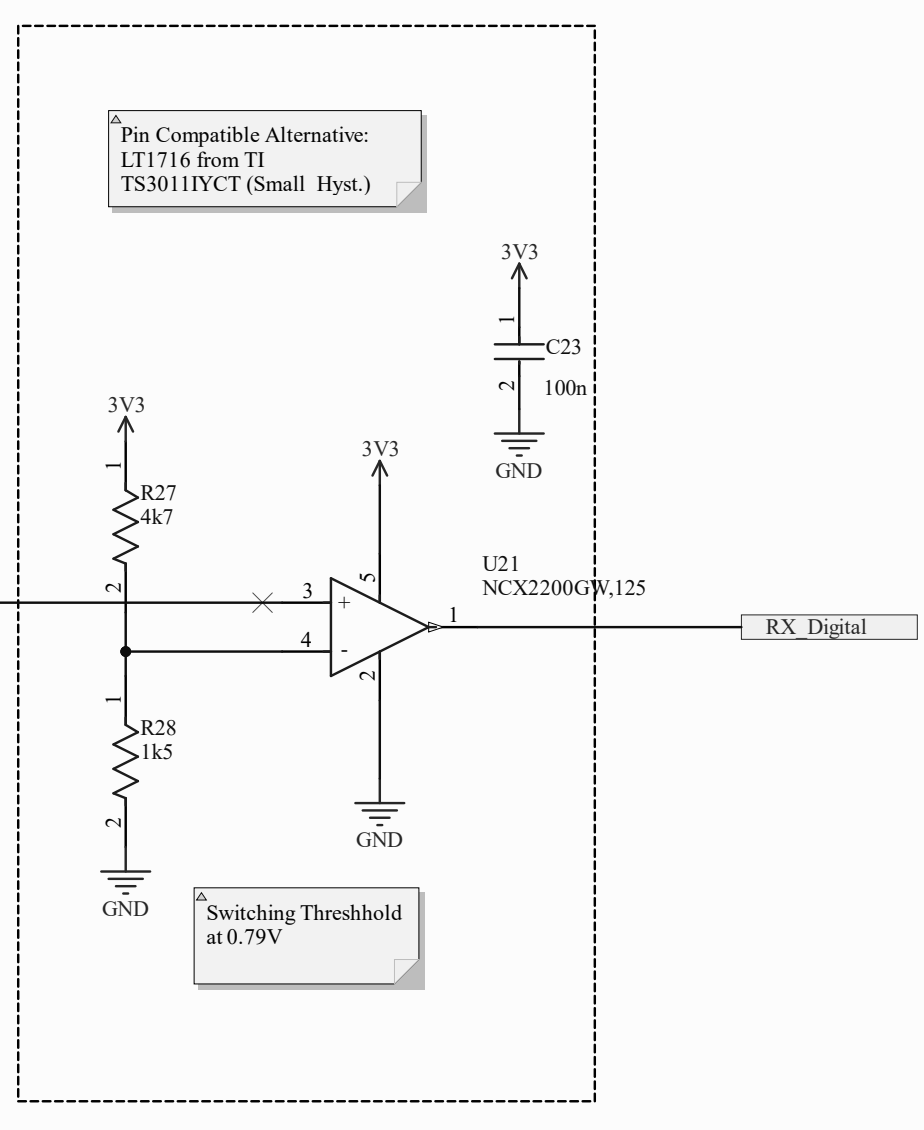
\includegraphics[width=0.4\textwidth]{Pictures/Komparator.png}
    \caption{Komparator-Schaltung}
    \label{fig:opamp_schaltung}
\end{figure}

Die Abbildung 2.5 stellt den Komparator dar, der dazu dient, das analoge verstärkte Signal $S_{BB}(t)$ in ein digitales Signal umzuwandeln für
eine nachfolgende digitale Verarbeitung. Der Komparator besteht aus einem Operationsverstärker (Typ NCX2200GW), einem Spannungsteiler aus zwei Widerständen
R27 und R28 und wird mit einer Betriebspannung von 3,3V betrieben. Die am nichtinvertierenden Eingang anliegende Signalspannung $S_{BB}(t)$ wird mit
einer Referenzspannung $U_{Ref}$ am invertierenden Eingang verglichen. Dieser Schaltschwellwert ergibt sich wie folgt:
\\
\begin{equation}
    U_{\text{Ref}} = \frac{R_{28}}{R_{27} + R_{28}} \cdot 3{,}3\,\text{V}
    = \frac{1{,}5\,\text{k}\Omega}{4{,}7\,\text{k}\Omega + 1{,}5\,\text{k}\Omega} \cdot 3{,}3\,\text{V}
    \approx 0{,}798\,\text{V}
\end{equation}\\
In Abhängigkeit von der Signalspannung $S_{BB}(t)$ wird der Ausgang des Komparators auf High oder Low gesetzt.
\[
S_{BB}(t) > 0{,}798\,\mathrm{V} \implies \text{HIGH}
\]
\[
S_{BB}(t) < 0{,}798\,\mathrm{V} \implies \text{LOW}
\]
Dadurch wird ein binäres digitales Ausgangssignal erzeugt, das von einem Computer weiterverarbeitet werden kann.
\[
S_{BB}(t) \rightarrow S_{RX}(t)
\]
Der Schaltschwellwert $U_{Ref}$ wurde so gewählt, dass groß genug Signale sicher erkannt werden. Dabei werden jedoch Rauschen und Störsignale ignoriert.